\section{Model-Based Results}
\label{sec:si_model_based}

This section presents results from model-based analyses that complement the design-based Monte Carlo simulation in the main text.

\subsection{Distributional Test Results}
\label{sec:si_distributional_tests}

We summarize adherence to normal and lognormal assumptions for daily means in Table~\ref{tab:shapiro} for all three networks. For \city{Lucknow} and \city{Dhaka}, the lognormal assumption is often more appropriate than the normal assumption, as indicated by a greater number of days with $p>0.05$. This difference is pronounced in \city{Lucknow}, where there are more sensors. The \city{Chicago} partial-year window rejects both simple parametric forms on most days, reflecting the large number of valid sensors per day and the sensitivity of Shapiro--Wilk tests at high $N^*$. Figure~\ref{fig:si_daily_distributions} shows empirical histograms on representative low, median, and high days in each city, alongside the normal and lognormal density fits. The \city{Chicago} daily distributions are typically narrower than the South Asian distributions, reflecting the lower concentration regime and tighter cross-sensor agreement in the calibrated Open Air network.

\begin{table}[ht]
\centering
\small
\begin{tabular}{lrrrrrr}
\toprule
 & \multicolumn{2}{c}{Dhaka} & \multicolumn{2}{c}{Lucknow} & \multicolumn{2}{c}{Chicago} \\
\cmidrule(lr){2-3}\cmidrule(lr){4-5}\cmidrule(lr){6-7}
 & $\mathcal{N}$ & $\log \mathcal{N}$ & $\mathcal{N}$ & $\log \mathcal{N}$ & $\mathcal{N}$ & $\log \mathcal{N}$ \\
\midrule
$p <0.01$ & 204 & 167 & 209 & 130 & 262 & 264 \\
$0.01 \leq p < 0.05$ & 52 & 58 & 49 & 37 & 5 & 2 \\
$0.05 \leq p < 0.10$ & 15 & 24 & 27 & 24 & 4 & 0 \\
$p \geq 0.10$ & 94 & 116 & 80 & 174 & 1 & 6 \\
Not tested & 0 & 0 & 0 & 0 & 1 & 1 \\
\bottomrule
\end{tabular}
\caption{Exact Shapiro--Wilk $p$-value counts for daily cross-sensor distributions under the normal distribution ($\mathcal{N}$) and the lognormal distribution ($\log \mathcal{N}$). Counts cover 365 daily distributions in \city{Dhaka} and \city{Lucknow}, and the nine-month \city{Chicago} window; the ``Not tested'' row records dates with too few valid values for the test.}
\label{tab:shapiro}
\end{table}


\begin{figure}[H]
 \centering
 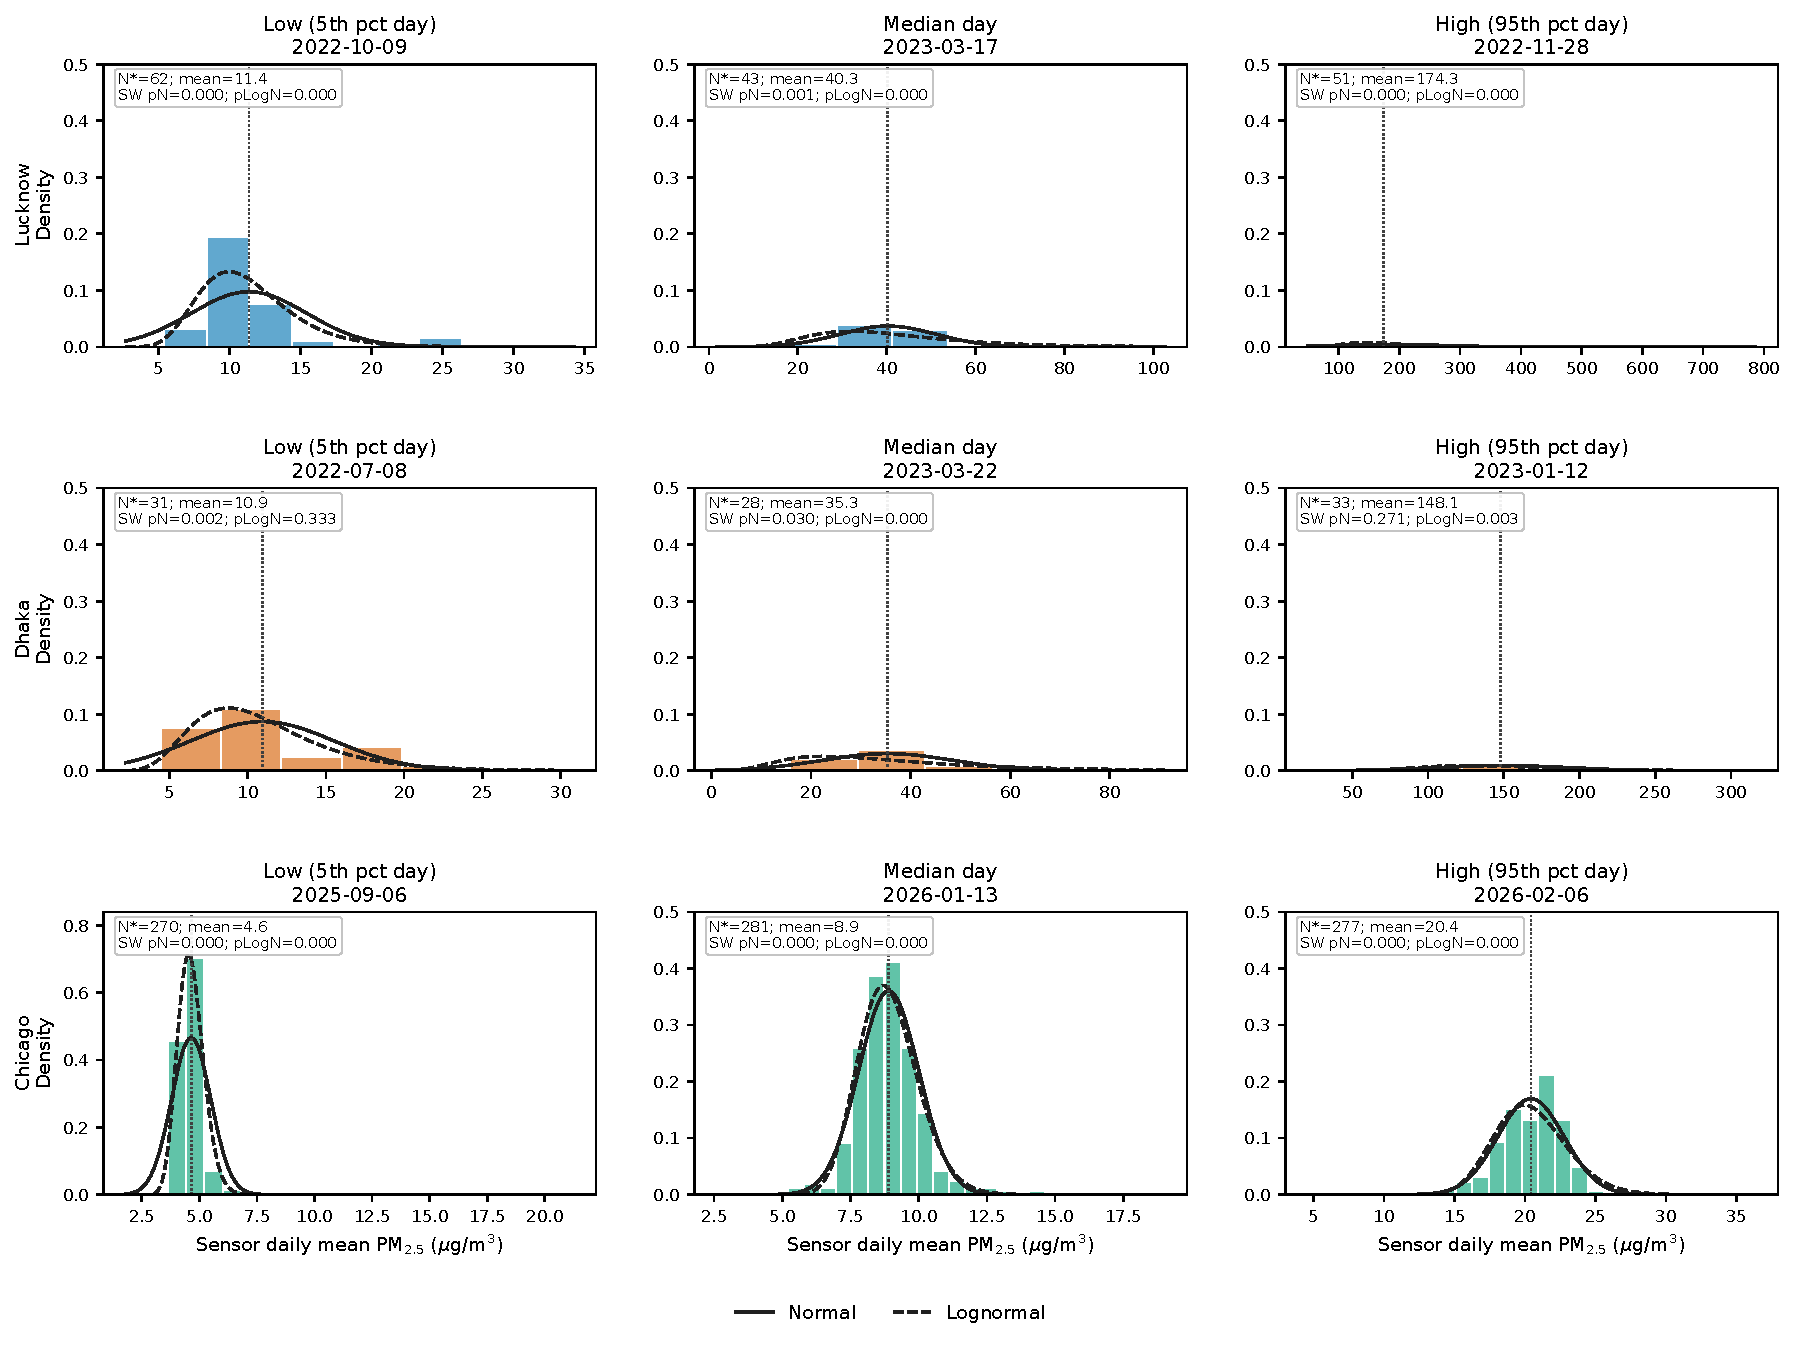
\includegraphics[width=0.98\textwidth]{Plots/Supporting_Information/Figure_SI_13/daily_distributions_representative_days.pdf}
 \caption{Empirical cross-sensor daily \pmtt\ distributions on representative low (5th percentile), median, and high (95th percentile) network-mean days for each city. Histograms show the density of valid sensor-level daily means; the solid black curve is a normal density fit and the dashed curve is a lognormal density fit. Dotted vertical lines mark the empirical mean. Shapiro--Wilk $p$-values for both fits are shown in each panel. Compared with the Q-Q plots in Figures~\ref{fig:moran_results} and~\ref{fig:hourly_qq}, these histograms make the cross-sectional skew visible directly and clarify why neither the normal nor the lognormal model is universally adequate, motivating the design-based MdAPE as the primary error metric.}
 \label{fig:si_daily_distributions}
\end{figure}

\subsection{RSE-Based Sample Size Estimates}
\label{sec:si_rse_results}

Using the RSE formulae derived in §\ref{sec:si_rse}, we calculate the number of sensors needed each day to achieve a target relative standard error, based on the sufficient statistics from each sensor network.

\subsubsection{Gaussian Results}
\label{sec:si_rse_gaussian}

In Figure~\ref{fig:appx_theor_gauss_ts}, we can see that the robust estimators for the daily means and standard deviations have a significant impact on the number of sensors needed per day to theoretically achieve less than 10\% error. Figures~\ref{fig:appx_theor_gauss_ts}--\ref{fig:lucknow_mu_sigma_hat} now show all three networks; \city{Chicago} should be interpreted as a partial-year transferability case rather than a full annual deployment.

\begin{figure}[H]
 \centering
 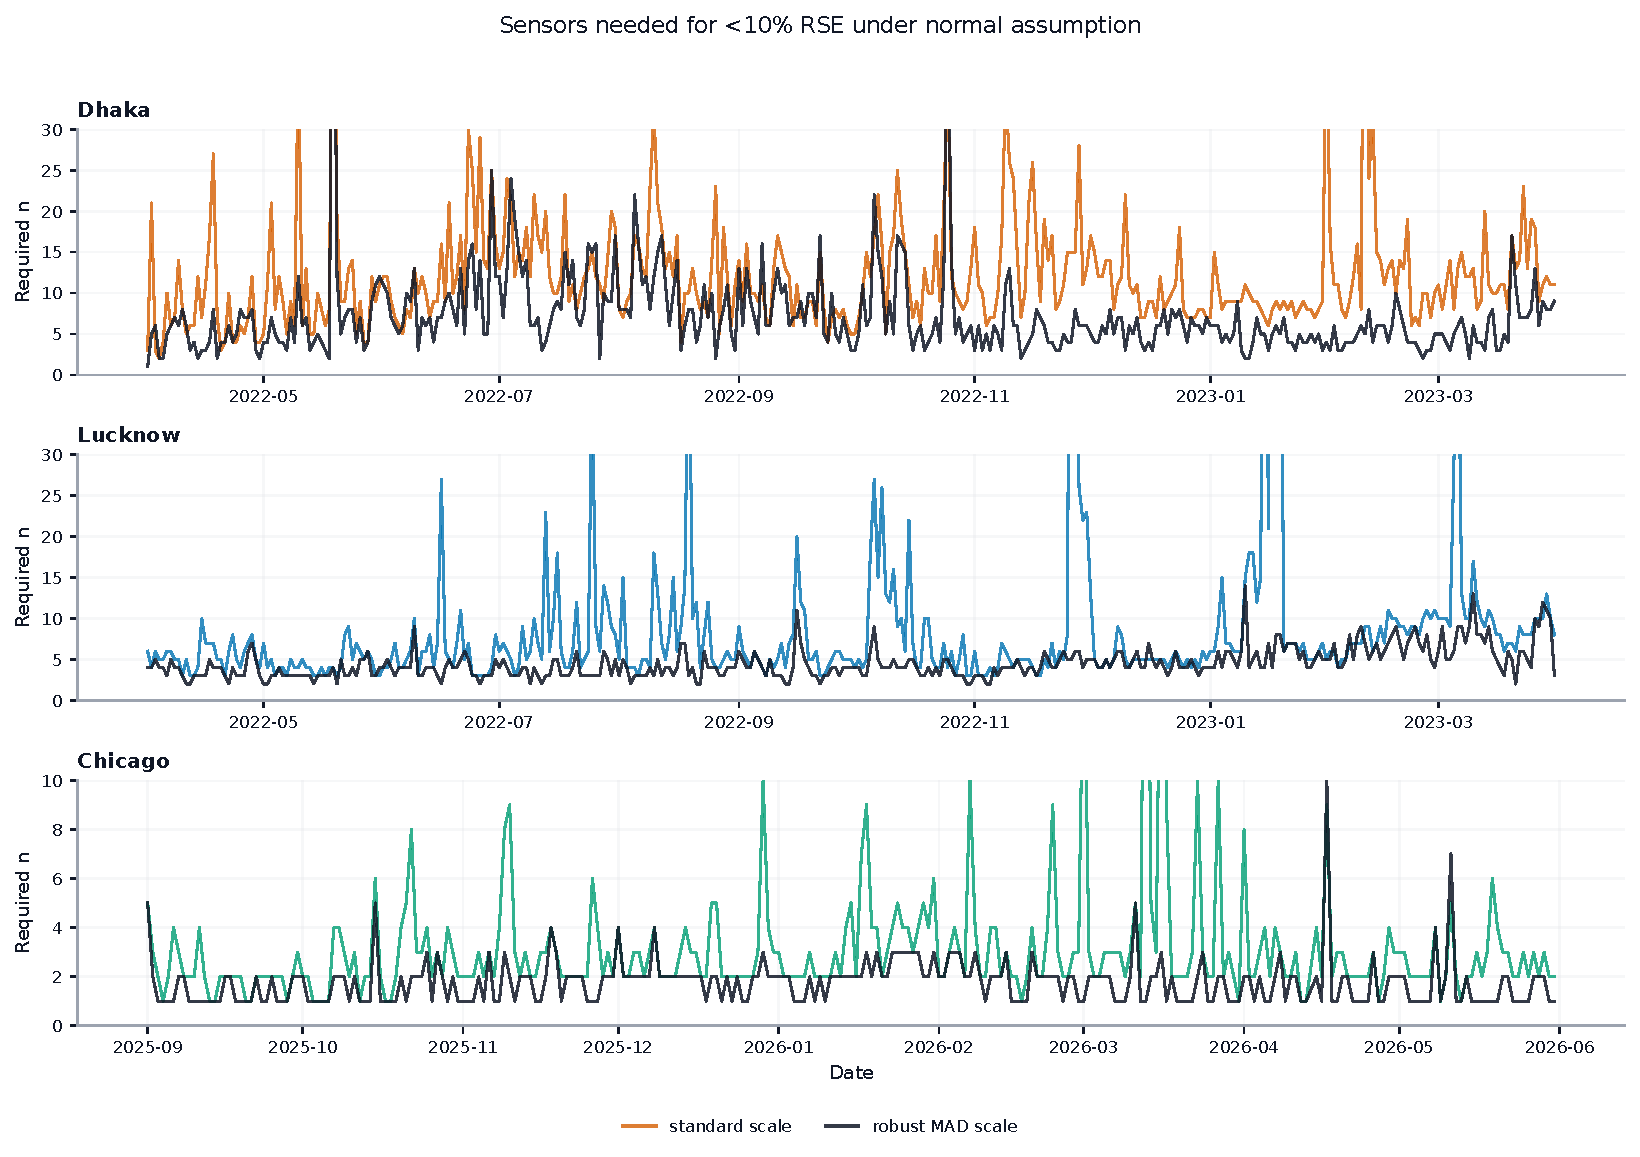
\includegraphics[width=0.95\textwidth]{Plots/Supporting_Information/Figure_SI_6/three_city_RSE_normal_daily_sensor_requirement.pdf}
 \caption{Time series of sensors required for a 10\% RSE threshold under the Gaussian assumption, for \city{Dhaka}, \city{Lucknow}, and \city{Chicago}. Panels use city-specific y-axis limits where needed so that the lower-concentration \city{Chicago} series remains readable.}
 \label{fig:appx_theor_gauss_ts}
\end{figure}

\subsubsection{Lognormal Results}
\label{sec:si_rse_lognormal_results}

We show the results for the log Normal estimator in Figure~\ref{fig:appx_theor_gauss_tslog}. Despite the log transform, we still see that the robust estimator diminishes the influence of potential outliers.

\begin{figure}[H]
 \centering
 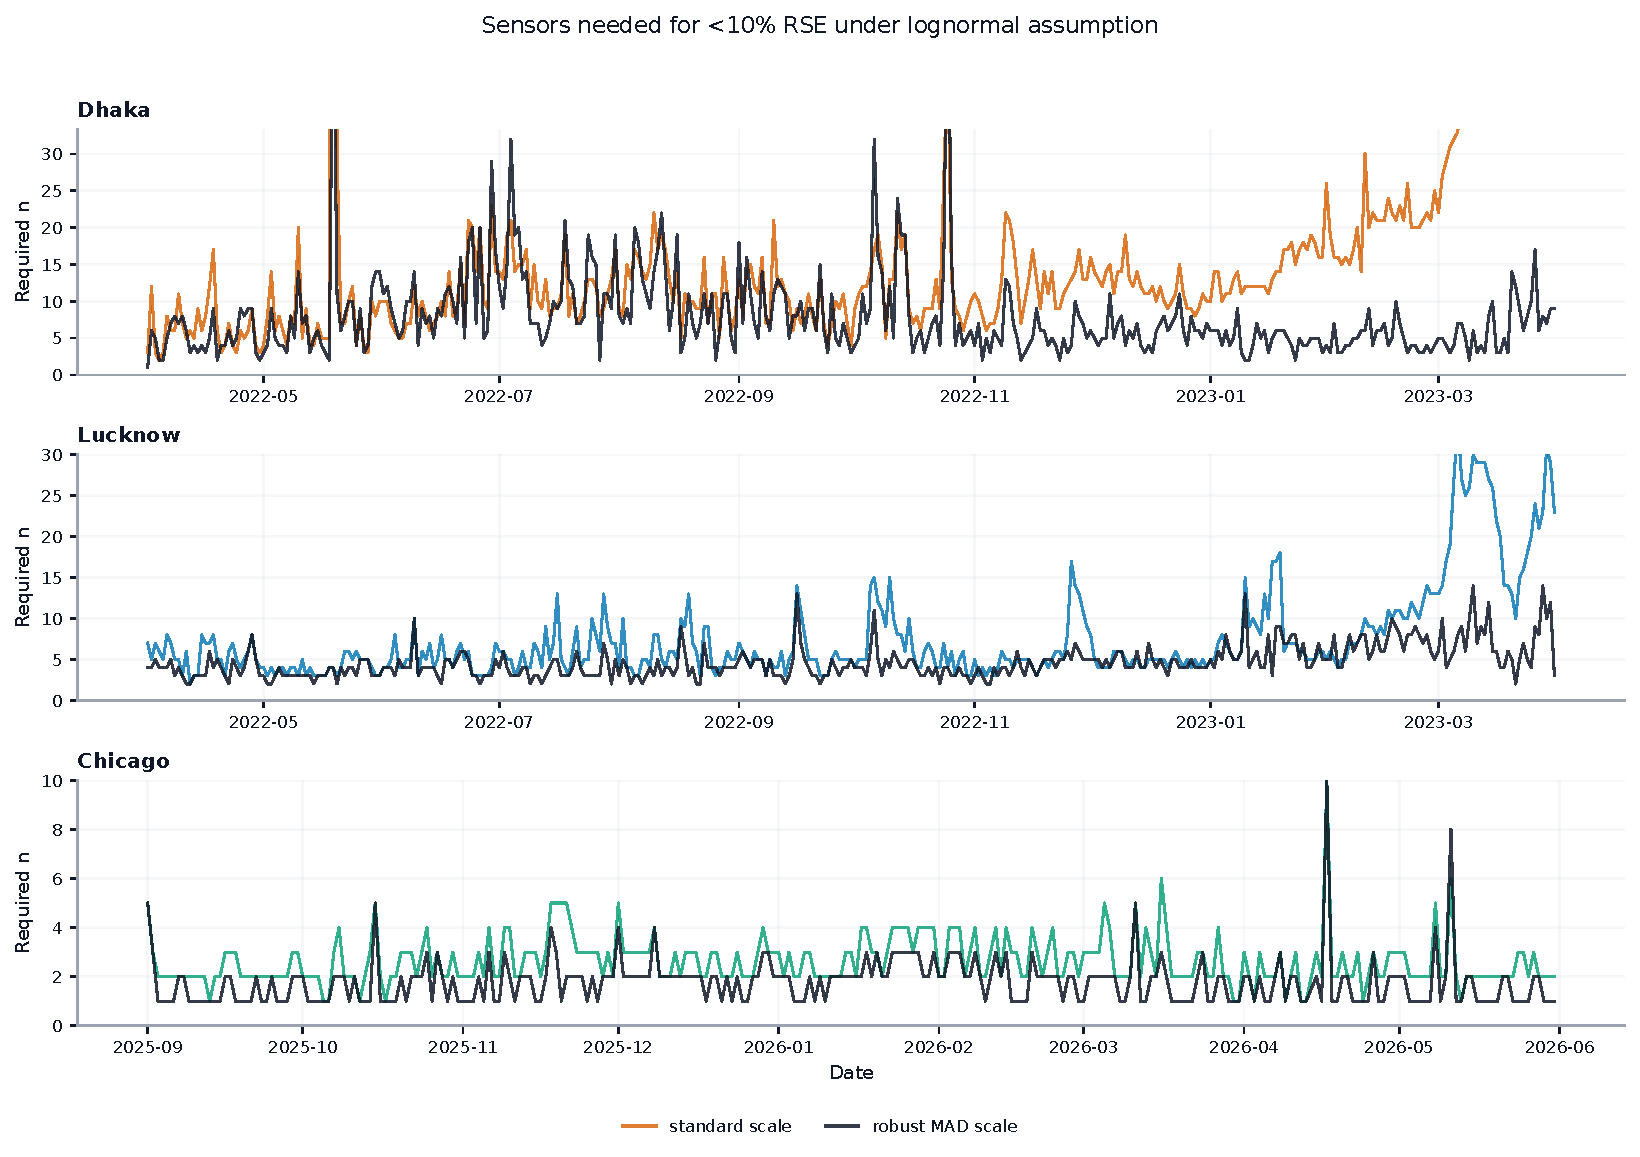
\includegraphics[width=0.95\textwidth]{Plots/Supporting_Information/Figure_SI_7/three_city_RSE_lognormal_daily_sensor_requirement.pdf}
 \caption{Time series of sensors required for a 10\% RSE threshold under the lognormal assumption, for \city{Dhaka}, \city{Lucknow}, and \city{Chicago}. Panels use city-specific y-axis limits where needed so that the lower-concentration \city{Chicago} series remains readable.}
 \label{fig:appx_theor_gauss_tslog}
\end{figure}

\subsubsection{Error Exceedance}
\label{sec:si_error_exceedance}

Given these results, the lognormal distribution is more likely to better describe the data distribution in the two South Asian networks. Figure~\ref{fig:err_exceed_10_main} plots, for each candidate subnetwork size $n$, the fraction of evaluated days for which the model-based RSE would remain above 10\%. The $n$-axis extends to 40 because the South Asian model-based RSE curves cross low-exceedance levels at substantially larger $n$ than the design-based MdAPE curves. Under the lognormal assumption, the figure suggests that the number of sensors needed for 10\% relative standard error is approximately 30--40 for \city{Dhaka} and 20--30 for \city{Lucknow}, depending on the tolerated fraction of exceedance days. However, given the $\delta^2$ term in the denominator of the RSE formulae, a threshold of $20\%$ would decrease this guidance by a factor of 4. The discrepancy between the two cities can be explained by the lognormal variance estimator. \city{Dhaka}'s lognormal variance estimator is consistently higher than the standard estimator; for \city{Lucknow}, the converse is true. Because we have fewer observations in \city{Dhaka}, this could indicate that the lognormal estimator provides a higher estimate of the variance with fewer samples.

\begin{figure}[H]
 \centering
 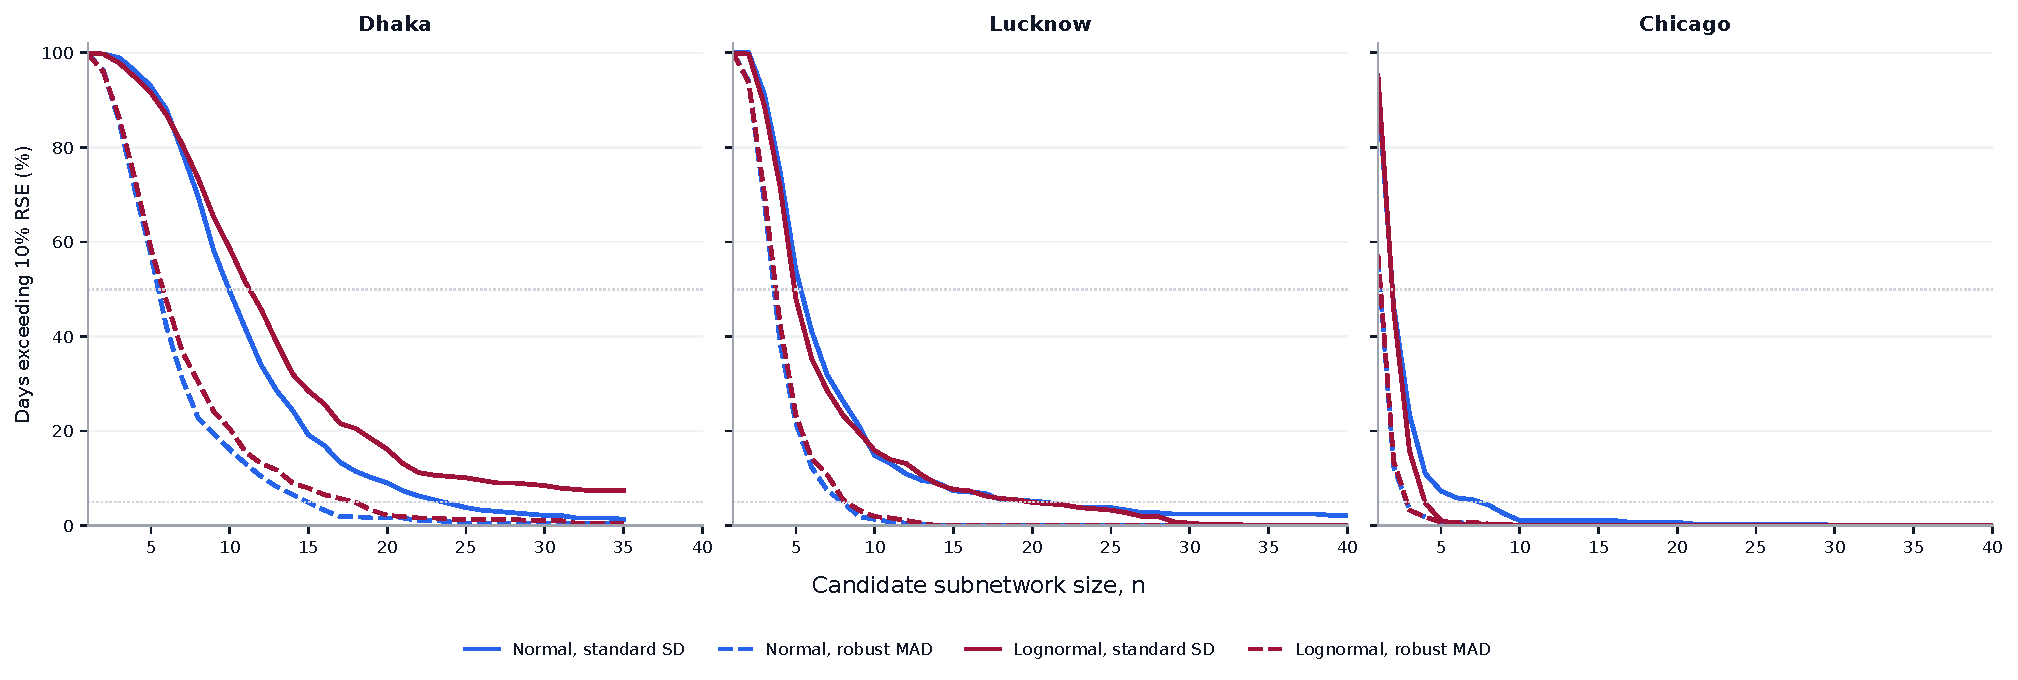
\includegraphics[width=0.95\textwidth]{Plots/Supporting_Information/Figure_SI_8/three_city_RSE_exceedance_curves.pdf}
 \caption{Fraction of evaluated days for which model-based RSE exceeds 10\%, plotted against candidate subnetwork size $n$ for \city{Dhaka}, \city{Lucknow}, and \city{Chicago}. The curves decrease monotonically as $n$ increases; the plotted range extends to $n=40$ because the South Asian RSE curves require larger candidate subnetworks than the MdAPE curves. The \city{Chicago} curve covers the nine-month deployment window and should be read as a partial-year transferability case.}
 \label{fig:err_exceed_10_main}
\end{figure}

For period means, $RSE < 10\%$ at 7 sensors for \city{Lucknow}, and 5 sensors for \city{Dhaka}. For the \city{Chicago} nine-month window, the analogous RSE requirement is met at very small $n$ (effectively $n = 2$--$3$), reflecting both the low inter-sensor variance in the Chicago calibrated dataset and the partial-year aggregation. The Chicago numbers should be treated as descriptive rather than as a full-year recommendation; the corresponding curves are reported in the released analysis outputs.


\subsubsection{Estimator Comparison}
\label{sec:si_estimator_comparison}

Across estimators in Figure~\ref{fig:err_exceed_10_main}, the robust Normal and robust lognormal results are similar, indicating that estimator choice matters more than the assumed distribution. This is consistent with the dispersion estimates shown in Figure~\ref{fig:lucknow_mu_sigma_hat}: the Normal model tends to yield larger $\hat{\sigma}$, whereas the lognormal model and robust estimators produce closer agreement, which directly drives the implied sensor requirements.

\begin{figure}[H]
 \centering
 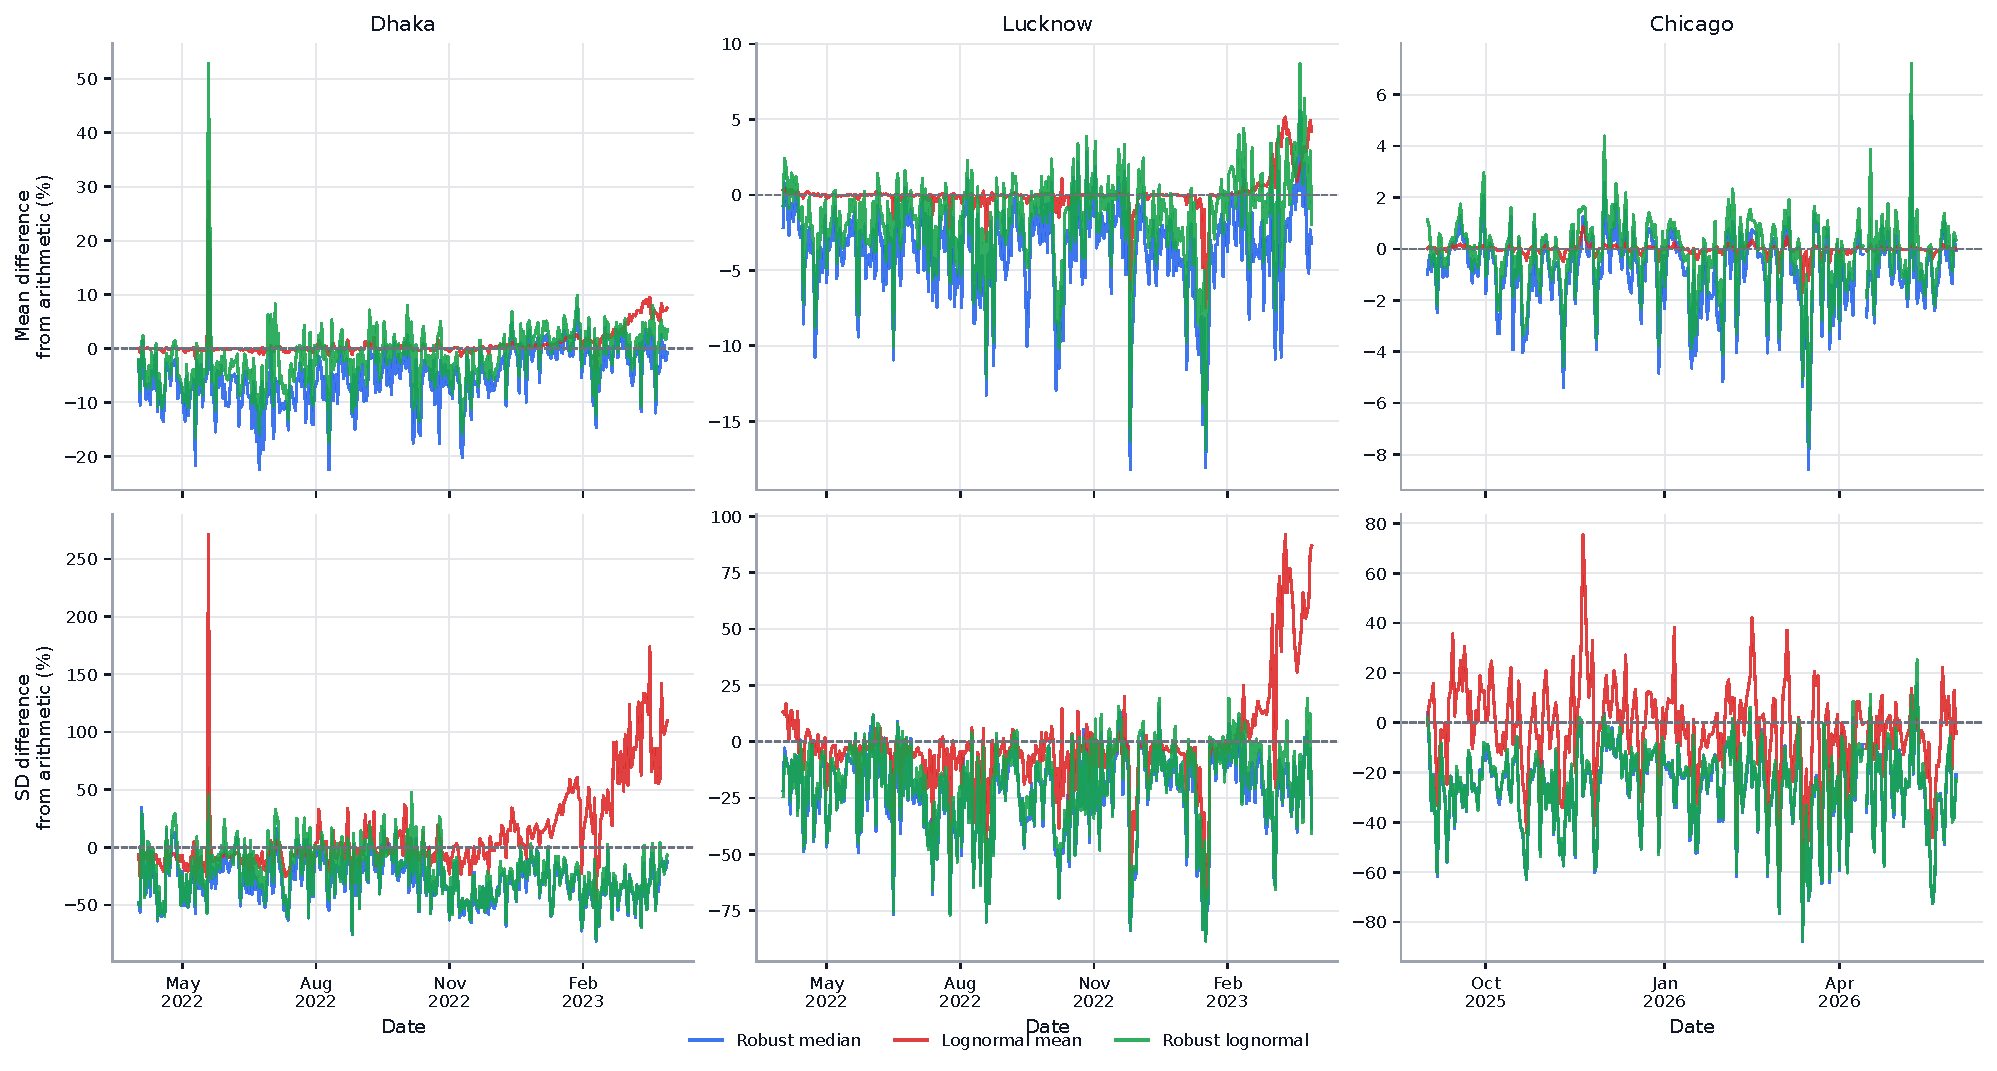
\includegraphics[width=0.95\textwidth]{Plots/Supporting_Information/Figure_SI_9/three_city_daily_estimator_mean_sd_comparison.pdf}
 \caption{Comparison of robust and lognormal estimators of daily cross-sensor $\hat{\mu}$ and $\hat{\sigma}$ relative to the arithmetic mean and standard deviation in \city{Dhaka}, \city{Lucknow}, and \city{Chicago}. The zero line corresponds to the arithmetic estimator used to define the reference-network mean.}
 \label{fig:lucknow_mu_sigma_hat}
\end{figure}
